% !TEX root = ../../main.tex

\subsection{OTFS-IM Error Decomposition}

The BER curves in the previous sections show the final end-to-end performance of OTFS-IM. However, total BER alone does not explain where the errors are produced inside the index-modulated receiver. In OTFS-IM, a detected bit can be wrong because the receiver selects an incorrect active-position pattern, because it detects an incorrect QAM symbol on an active position, or because both events occur in the same IM block. Therefore, this section decomposes the OTFS-IM result into index BER, symbol BER, and pattern error rate.

The decomposition is especially useful for interpreting whether the performance of a pattern-selection method is limited by the geometry of the selected activation patterns or by the reliability of the symbol decisions after the active positions have already been estimated. In the simulation, the index BER is computed from the recovered pattern bits, the symbol BER is computed from the recovered QAM bits on the active positions, and the pattern error rate measures the probability that the active-position pattern of an IM block is detected incorrectly.

\IfFileExists{Images/Chapter5/error_decomposition_n6_k5.png}{%
\begin{figure}[H]
    \centering
    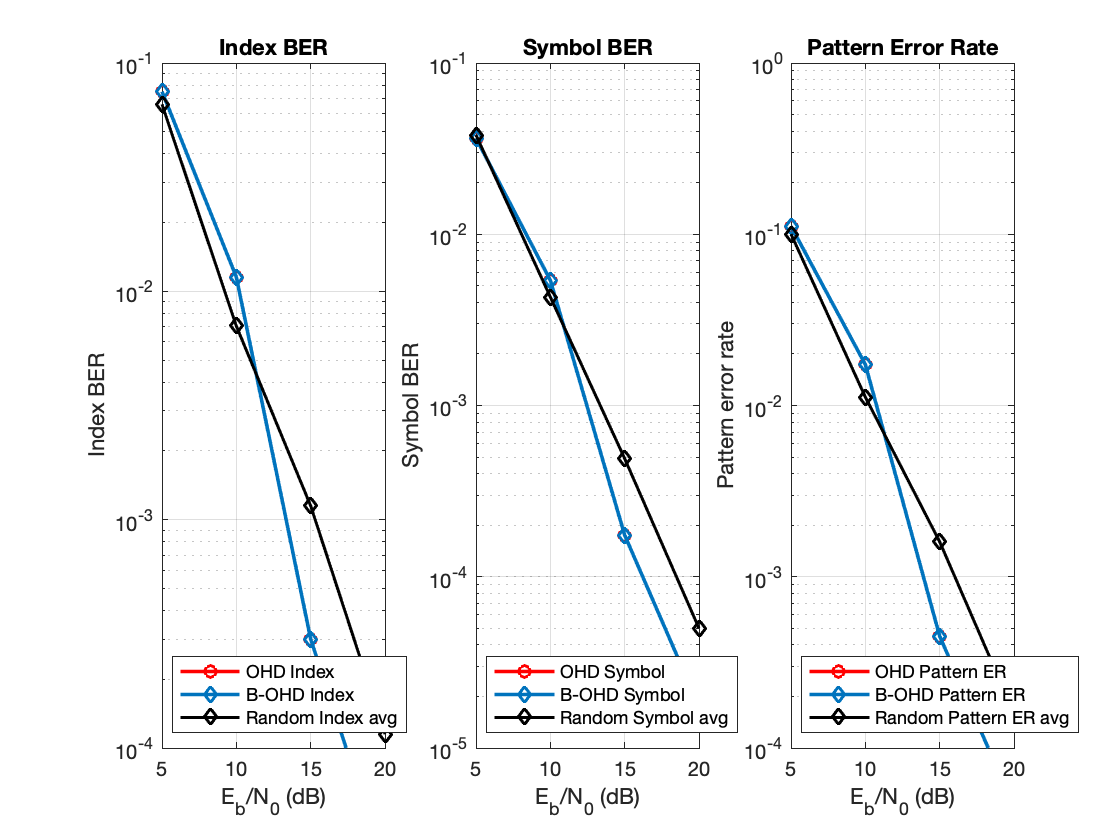
\includegraphics[width=0.95\linewidth]{Images/Chapter5/error_decomposition_n6_k5.png}
    \caption{Error decomposition of OHD and B-OHD OTFS-IM for \(n=6,k=5\)}
    \label{fig:chapter5_error_decomposition_n6_k5}
\end{figure}
}{%
\begin{figure}[H]
    \centering
    \fbox{%
        \begin{minipage}[c][0.25\textheight][c]{0.88\linewidth}
            \centering
            Required figure file is missing:\\
            Images/Chapter5/error\_decomposition\_n6\_k5.png
        \end{minipage}
    }
    \caption{Error decomposition of OHD and B-OHD OTFS-IM for \(n=6,k=5\)}
    \label{fig:chapter5_error_decomposition_n6_k5}
\end{figure}
}

Figure~\ref{fig:chapter5_error_decomposition_n6_k5} presents the error decomposition for the equal-spectral-efficiency configuration \(n=6,k=5\). This configuration is selected because it was used as the main equal-SE case in the previous section, where OTFS-IM and baseline OTFS both transmit \(2.00\) bits per resource element. As a result, the decomposition can be interpreted without the ambiguity of a rate advantage or a rate penalty.

At low SNR, both the index and symbol components are relatively large. This behavior is expected because the MP detector receives unreliable soft information from the delay-Doppler grid. Under this condition, the receiver may confuse the active positions and may also assign incorrect QAM symbols to positions that are detected as active. Therefore, the BER of OTFS-IM is not yet clearly separated into a purely index-limited or purely symbol-limited regime.

At medium SNR, the decomposition becomes more informative. For the \(n=6,k=5\) case, the OHD and B-OHD pattern tables are identical in the implemented simulation, so the two curves overlap. At \(E_b/N_0=10~\mathrm{dB}\), the total BER is approximately \(6.41\times10^{-3}\), while the measured index BER and symbol BER are approximately \(1.16\times10^{-2}\) and \(5.39\times10^{-3}\), respectively. In the bit-level contribution reported by the simulation, the symbol component accounts for about \(70\%\) of the total erroneous bits and the index component accounts for about \(30\%\). This means that, although pattern detection is important, the final BER is also strongly affected by the reliability of QAM symbol decisions on the detected active positions.

The pattern error rate provides a complementary view. At \(10~\mathrm{dB}\), the pattern error rate is approximately \(1.74\times10^{-2}\), which is higher than the total BER because one wrong pattern event is counted at the block level rather than at the bit level. A single pattern error does not necessarily imply that all bits in the IM block are wrong. Some symbol bits may still be recovered correctly, and some wrong active-position decisions may affect only part of the index-bit representation. For this reason, pattern error rate should not be compared directly with total BER as if they were the same metric. It is better interpreted as a diagnostic indicator of active-position reliability.

At higher SNR, the index and symbol components both decrease sharply. In the reported \(n=6,k=5\) result, the OTFS-IM BER approaches the Monte Carlo resolution at \(20~\mathrm{dB}\), and both index and symbol BER become nearly zero. This confirms that the detector is able to exploit the delay-Doppler representation effectively when the noise level is sufficiently low. It also shows that the performance gain observed in the BER curves is not produced by only one part of the receiver. Instead, it comes from the combined improvement in active-pattern detection and active-symbol detection.

The main conclusion from this decomposition is that OTFS-IM performance is jointly limited by pattern reliability and symbol reliability. Pattern selection can reduce the probability of confusing activation patterns, but it cannot fully determine the BER by itself. Once the active pattern is detected with reasonable reliability, the remaining errors are increasingly dominated by the QAM decisions on the active positions. This observation is important for the following section, where deterministic pattern selection is compared with random pattern selection. A good pattern table is beneficial, but its advantage is configuration-dependent and must be evaluated together with the detector behavior and the operating SNR range.
